\chapter{Implementation}

\section{The Tool used}
JBotSim is an open source simulation library that is dedicated
to distributed algorithms in dynamic networks. I developed it with
the purpose in mind to make it possible to implement an algorith-
mic idea in minutes and interact with it while it is running (e.g.,
add, move, or delete nodes). Besides interaction, JB OT S IM can
also be used to prepare live demos of an algorithm and to show it
to colleagues or students, as well as to assess the algorithm per-
formance. JB OT S IM is not a competitor of mainstream simulators
such as NS3 [5], OMNet [10], or The One [8], in the sense that it
does not aim to implement real-world networking protocols. Quite
the opposite, JB OT S IM aims to remain technology-insensitive and
to be used at the algorithmic level, in a way closer in spirit to the
ViSiDiA project (a general-purpose platform for distributed algo-
rithms). Unlike ViSiDiA, however, JB OT S IM natively supports
mobility and dynamic networks (as well as wireless communica-
tion). Another major difference with the above tools is that it is a
library rather than a software: its purpose is to be used in other pro-
grams, whether these programs are simple scenarios of full-fledged
software. Finally, JB OT S IM is distributed under the terms of the
LGPL licence, which makes it easily extensible by the community.
Whether the algorithms are centralized or distributed, the natu-
ral way of programming in JB OT S IM is event-driven: algorithms
are specified as subroutines to be executed when particular events
occur (appearance or disappearance of a link, arrival of a message,
clock pulse, etc.). Movements of the nodes can be controlled ei-
ther by program or by means of live interaction with the mouse
(adding, deleting, or moving nodes around with left-click, right-
click, or drag and drop, respectively). These movements are typi-
cally performed while the algorithm is running, in order to visualize
it or test its behavior in challenging configurations.
The present document offers a broad view of JB OT S IM ’s main
features and design traits. I start with preliminary information in
Section 2 regarding installation and documentation. Section 3 re-
views JB OT S IM ’s main components and specificities such as pro-
gramming paradigms, clock scheduling, user interaction, or global
architecture. Section 4 zooms on key features such as the exchange
of messages between nodes, graph-level APIs, or the creation of
online demos. Finally, I discuss in Section 5 some extensions of
JB OT S IM , including TikZ exportation feature and edge-markovian
dynamic graph generator.
Besides its features, the main asset of JBotSim is its simplicity
of use – an aim that I pursued at the cost of re-writing it several
times from scratch (the API is now stable).
\section{Features and Architecture}
This section provides an overview of JB OT S IM ’s key features
and discusses the reason why some design choices were made. I
review topics as varied as programming paradigms, clock schedul-
ing, user interaction, and global architecture.
\subsection{Basic features of nodes and links}

\begin{figure}[hbtp]
\centering
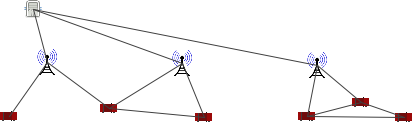
\includegraphics[scale=1]{screenshot_4.png}
\caption{A highway scenario composed of vehicles, road-side
units, and central servers. Part of the network is ad hoc (and
wireless); the rest is infrastructured (and wired)}
\end{figure}

JB OT S IM consists of a small number of classes, the most cen-
tral being Node, Link, and Topology. The contexts in which
dynamic networks apply are varied. In order to accommodate a
majority of cases, these classes offer a number of conceptual varia-
tions around the notions of nodes and links. Nodes may or may not
possess wireless communication capabilities, sensing abilities, or
self-mobility. They may differ in clock frequency, color, commu-
nication range, or any other user-defined property. Links between
the nodes account for potential communication among them. The
nature of links varies as well; a link can be directed or undirected,
as well as it can be wired or wireless – in the latter case JB OT S IM ’s
topology will update the set of links automatically, as a function of
nodes distances and communication ranges.
Figures 1 and 2 illustrate two different contexts. Figure 1 depicts
a highway scenario where three types of nodes are used: vehicles,
road-side units (towers), and central servers. This scenario is semi-
infrastructured: Servers share a dedicated link with each tower.
These links are wired and thus exist irrespective of distance. On
the other hand, towers and vehicles communicates through wire-
less links that are automatically updated.

\begin{figure}[hbtp]
\centering
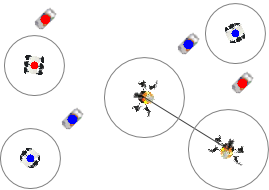
\includegraphics[scale=1]{screenshot_5.png}
\caption{A swarming scenario, whereby mobiles robots and
UAVs collaborate in order to clean a public park}
\end{figure}

Figure 2 illustrates a purely ad hoc scenario, whereby a hetero-
geneous swarm of UAVs and robots strives to clean a public park
collectively. In this scenario, robots can detect and clean wastes
of a certain type (red or blue) only if these are within their sens-
ing range (depicted by a surrounding circle). However, they are
pretty slow to move and cannot detect remote wastes. In the mean-
time, a set of UAVs is patrolling over the park at higher speed and
with larger sensing range. Whenever they detect a waste of some
type, they store its position and start searching for a capable robot.
In addition to sensing capabilities, UAVs can exchange messages
with each other to optimize the process.
Besides nodes and links, the concept of topology is central in
JB OT S IM . Topologies can be thought of as containers for nodes
and links, together with dedicated operations like updating wireless
links. They also play a central role in JB OT S IM ’s event architec-
ture, as explained later on.

\subsection{Distributed vs. centralized algorithms}
JB OT S IM supports the manipulation of centralized or distributed
algorithms (possibly simultaneously). The natural way to imple-
ment a distributed algorithm is by extending the Node class, in
which the desired behavior is implemented. Centralized algorithms
are not constrained to a particular model, they can take the form of
any standard java class.
\textit{Distributed Algorithm}
JB OT S IM comes with a default type of node that is implemented
in the Node class. This class provides the most general features
a node could have, including primitives for moving, exchanging
messages, or tuning basic parameters (e.g. communication range
and sensing range). Distributed algorithms are naturally imple-
mented through adding specific features to this class. Listing 2
provides a basic example in which the nodes are endowed with
self-mobility. The class relies on a key mechanism in JB OT S IM :
performing periodic operations that are triggered by the pulse of the
system clock. This is done by overriding the onClock() method,
which is called periodically by JBotSim’s engine (by default, at
every pulse of the clock). The rest of the code is responsible for
moving the node, setting a random direction at construction time
(in radian), then moving in this direction periodically. (More de-
tails about the movement API can be found online.)
\subsection{Architecture of the event system}
So far, we have seen one type of event: clock pulses, to be lis-
tened to through the ClockListener interface. JB OT S IM offers
a number of such events and interfaces, some of which become are
ubiquitous. The main ones are depicted on Figure 3 on the fol-
lowing page. This architecture allows one to specify dedicated op-
erations in reaction to various events. For instance, one may ask
to be notified whenever a link appears or disappears somewhere.
Same for messages, which are typically listened to by the nodes
themselves or can be watched at a global scale (e.g. to keep a log
of all communications). In fact, every node is automatically noti-
fied for its own events; it just needs to override the corresponding
methods from the parent class Node in order to specify event han-
dlings (e.g. onClock(), onMessage(), onLinkAdded(),
onSensingIn(), onSelection(), etc.). Explicit listeners,
on the other hand, like the ones in Figure 3, are meant to be used
by centralized programs which do not extend class Node.
Listing 6 gives one such example, consisting of a mobility trace
recorder. This program listens to topological events of various
kinds, including appearance or disappearance of nodes or links, and
movements of the nodes. Upon each of these events, it outputs a
string representation of the event using a dedicated human readable
format called DGS [7]. Similar code could be written for Gephi [3].
Other events exist besides those represented in Figure 3, such
as the SelectionListener interface, which makes it possible
to be notified when a node is selected (middle-click) and make it
initiate some tasks, for instance broadcast, distinguished role, etc.
\subsection{Single threading: why and how?}
It seems convenient at first, to assign every node a dedicated
thread, however JB OT S IM was designed differently. JB OT S IM is
single-threaded, and definitely so. This section explains the why
and the how. Understanding these aspects are instrumental in de-
veloping well-organized and bug-free programs.
In JB OT S IM , all the nodes, and in fact all of JB OT S IM ’s life
(GUI excepted) is articulated around a single thread, which is driven
by the central clock. The clock pulses at regular interval (whose
period can be tuned) and notifies its listeners in a specific order.
JB OT S IM ’s internal engines, such as the message engine, are served
first. Then come those nodes whose wait period has expired (re-
mind that nodes can choose to register to the clock with different
periods). These nodes are notified in a random order. Hence, if
all nodes listen to the clock at a rate of 1 (the default value), they
will all be notified in a random order in each round, which makes
JB OT S IM ’s scheduler a non-deterministic 2-bounded fair sched-
uler. (Other policies will be available eventually.) A simplified
version of the current scheduling process is depicted on Figure 4.
One consequence of single-threading is that all computations
(GUI excepted) take place in a sequential order that makes it pos-
sible to use unsynchronized data structures and simpler code. This
also improves the scalability of JB OT S IM when the number of
nodes grows large. One can rely on other user-defined threads in
the program, however one should be careful that these thread do not
interfer with JB OT S IM ’s. The canonical example is when a sce-
nario is set up by program from within the thread of the main()
method. If the initialization makes extensive use of JB OT S IM ’s
API from within that thread and the clock starts triggering events
at the same time, then problems might occur (and a Concurrent
ModificationException be raised). The easy way around
is to pause the clock before executing these instructions and to re-
sume it after (using the pause() and the resume() methods on
the topology, respectively).
\subsection{Interactivity}
I designed JB OT S IM with a clear separation in mind between
GUI and internal features. In particular, it can be run without GUI
(i.e. without creating the JViewer object), and things will work
exactly the same, though invisibly. As such, JB OT S IM can be used
to perform batch simulations (e.g. sequences of unattended runs
that log the effects of some varying parameter). This also enables
to withstand heavier simulations in terms of the number of nodes
and links.
This being said, one of the most distinctive features of JB OT S IM
remains interactivity, e.g., the ability to challenge the algorithm in
difficult configurations through adding, removing, or moving nodes
during the execution. This approach proves useful to think of a
problem visually and intuitively. It also makes it possible to explain
someone an algorithm through showing its behavior.
The architecture of JB OT S IM ’s viewer is depicted on Figure 5.
As one can see, the viewer relies heavily on events related to nodes,
links, and topology. The influence also goes the other way, with
mouse actions being translated into topological operations. These
features are realized by a class called JTopology. This class
can often be ignored by the developer, which creates and manip-
ulates the viewer through the higher JViewer class. The latter
adds external features such as tuning slide bars, popup menus, or
self-containment in a system window.
While natural to JB OT S IM ’s users, the viewer remains, in all
technical aspects, an independent piece of software. Alternative
viewers could very well be designed with specific uses in mind.

\begin{figure}[hbtp]
\centering
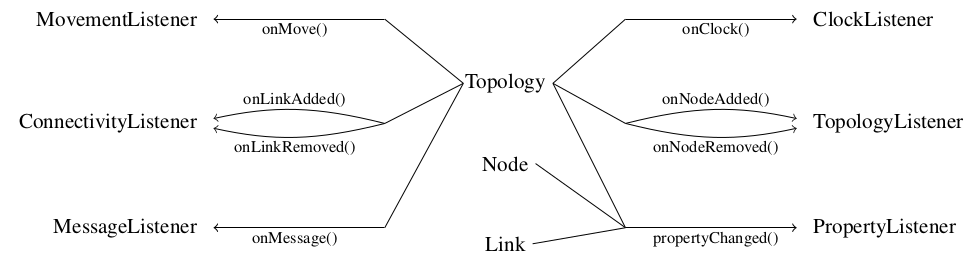
\includegraphics[scale=1]{screenshot_6.png}
\caption{Main sources of events and corresponding interfaces in JB OT S IM}
\end{figure}
